\chapter{Background}
This chapter provides background information on Wireless Networks and recalls some graph-theoretic basics we use for our purposes.

At first we will take a close look at the modes of operation of wireless accesspoints followed by the bigger picture on how to use these accesspoints
within a wireless mesh network. Then we examine the way accesspoints communicate with each other through channels, how those communications are affected by interference and
how they deal with accessing the shared medium. Finally we will outline the implementation of the \ac{WDS} we want to optimize and emphasize where it differs from a common
\ac{WDS}.

In the second part we shortly explain spanning trees on graphs and illustrate graph attributes like edge and vertex connectivities.
Subsequently we will give a detailed description of how we map our real world \ac{AP}-infrastructe-setups to network graphs in order to compute solutions and conclude this part by
discussing the relevance of the problem COLORING for our approach.

\section{Wireless Networks}
  Wireless networks are computer networks which use radio-waves instead of cables in order two communicate.
  They are used in scenarios where using wires for connections are not possible or cumbersome like systems where devices are mobile.
  There are different scales where wireless connections are utilized:
    \begin{itemize}
      \item Smallish systems like a \ac{PAN} where a smartphone would use bluetooth to connect to headphones or glasses. Typical range for this field of
	application is within a few meters.
      \item Medium Sized systems like a \ac{WLAN} with laptops or smartphones connecting to an infrastructure through a wireless accesspoint.
	Typical range is about 50 meters.
      \item Large scale systems like television broadcasting with \ac{DVB-T} through satellites with typical ranges of up to 35400 kilometers.
    \end{itemize}
  \subsection{Wireless Access-Point}
    A Wireless Access-Point is a device which allows other devices with wireless adapters to connect to its network.
    Mostly it serves as an entry point to a network-infrastructure and ultimately the internet like a common network switch, 
    but accesspoints have more modes of operation. Those are in general the following
    \begin{description}
      \item[Infrastructure-mode]
	Using this mode, the clients connect themselves to the accesspoints in order to get access to the network behind the accesspoints, like fileservers or the internet.
	To do so one or more accesspoints announce their services through small broadcasted packets called beacons, which include a \ac{SSID}, 
	the name/identifier of the wireless network. This is done 
	so that multiple wireless networks can be differentiated from each other. Those SSIDs, if received, are then used by the clients to
	establish a link to the herein before mentioned accesspoints.
      \item [Ad-hoc-mode]
	In an ad-hoc network all participants (accesspoints and clients) use the same \ac{SSID} and create spontaneous connections between each other in order to 
	exchange data. Note that also the former end-user-devices like laptops or smartphones are now nodes in this network and route packets instead of just originating or
	terminating them. \cite{Akyildiz2005445}.
     \item [Client-mode]
	Here the accesspoint acts the same as the wireless adapter of ordinary end-user-devices and establish links to other infrastructure-serving accesspoints or 
	ad-hoc systems. For example a laptop could be connected to an accesspoint through wire and then this accesspoint connects iteself to another network.
    \end{description}
    
    \begin{figure}[h!]
      \centerline{
	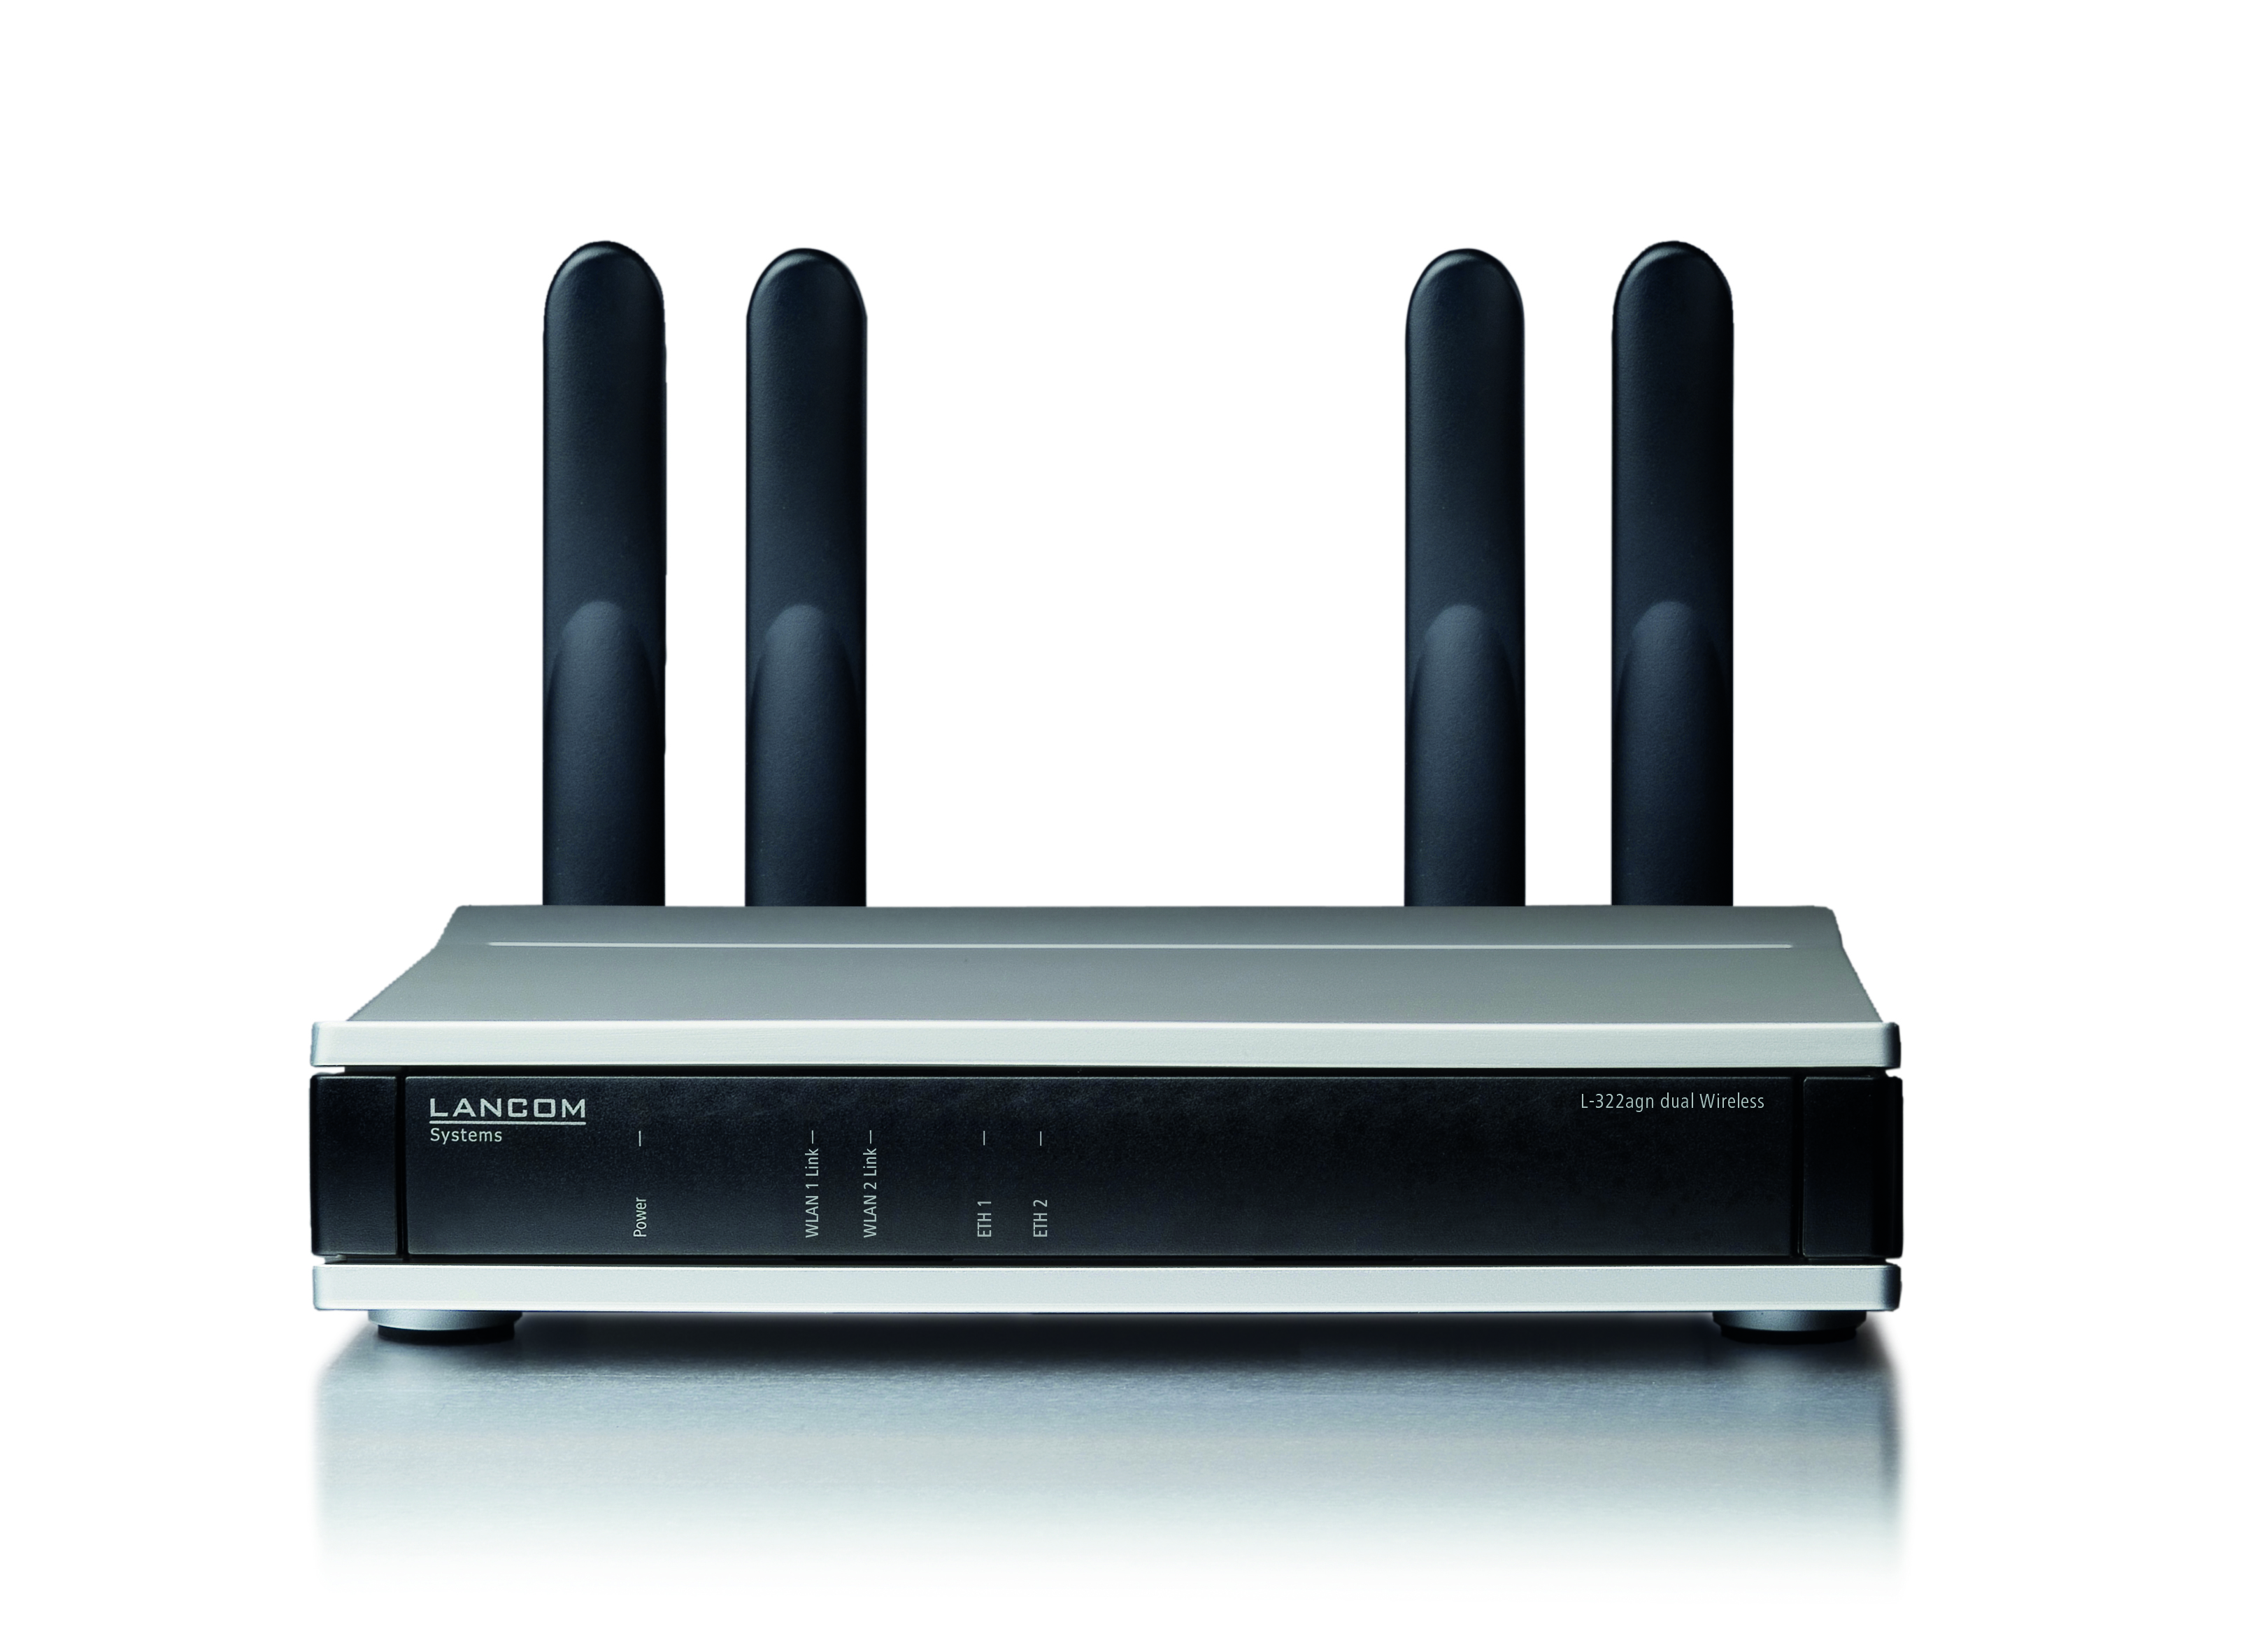
\includegraphics[width=0.5\textwidth]{figures/L-322agn.jpg}
	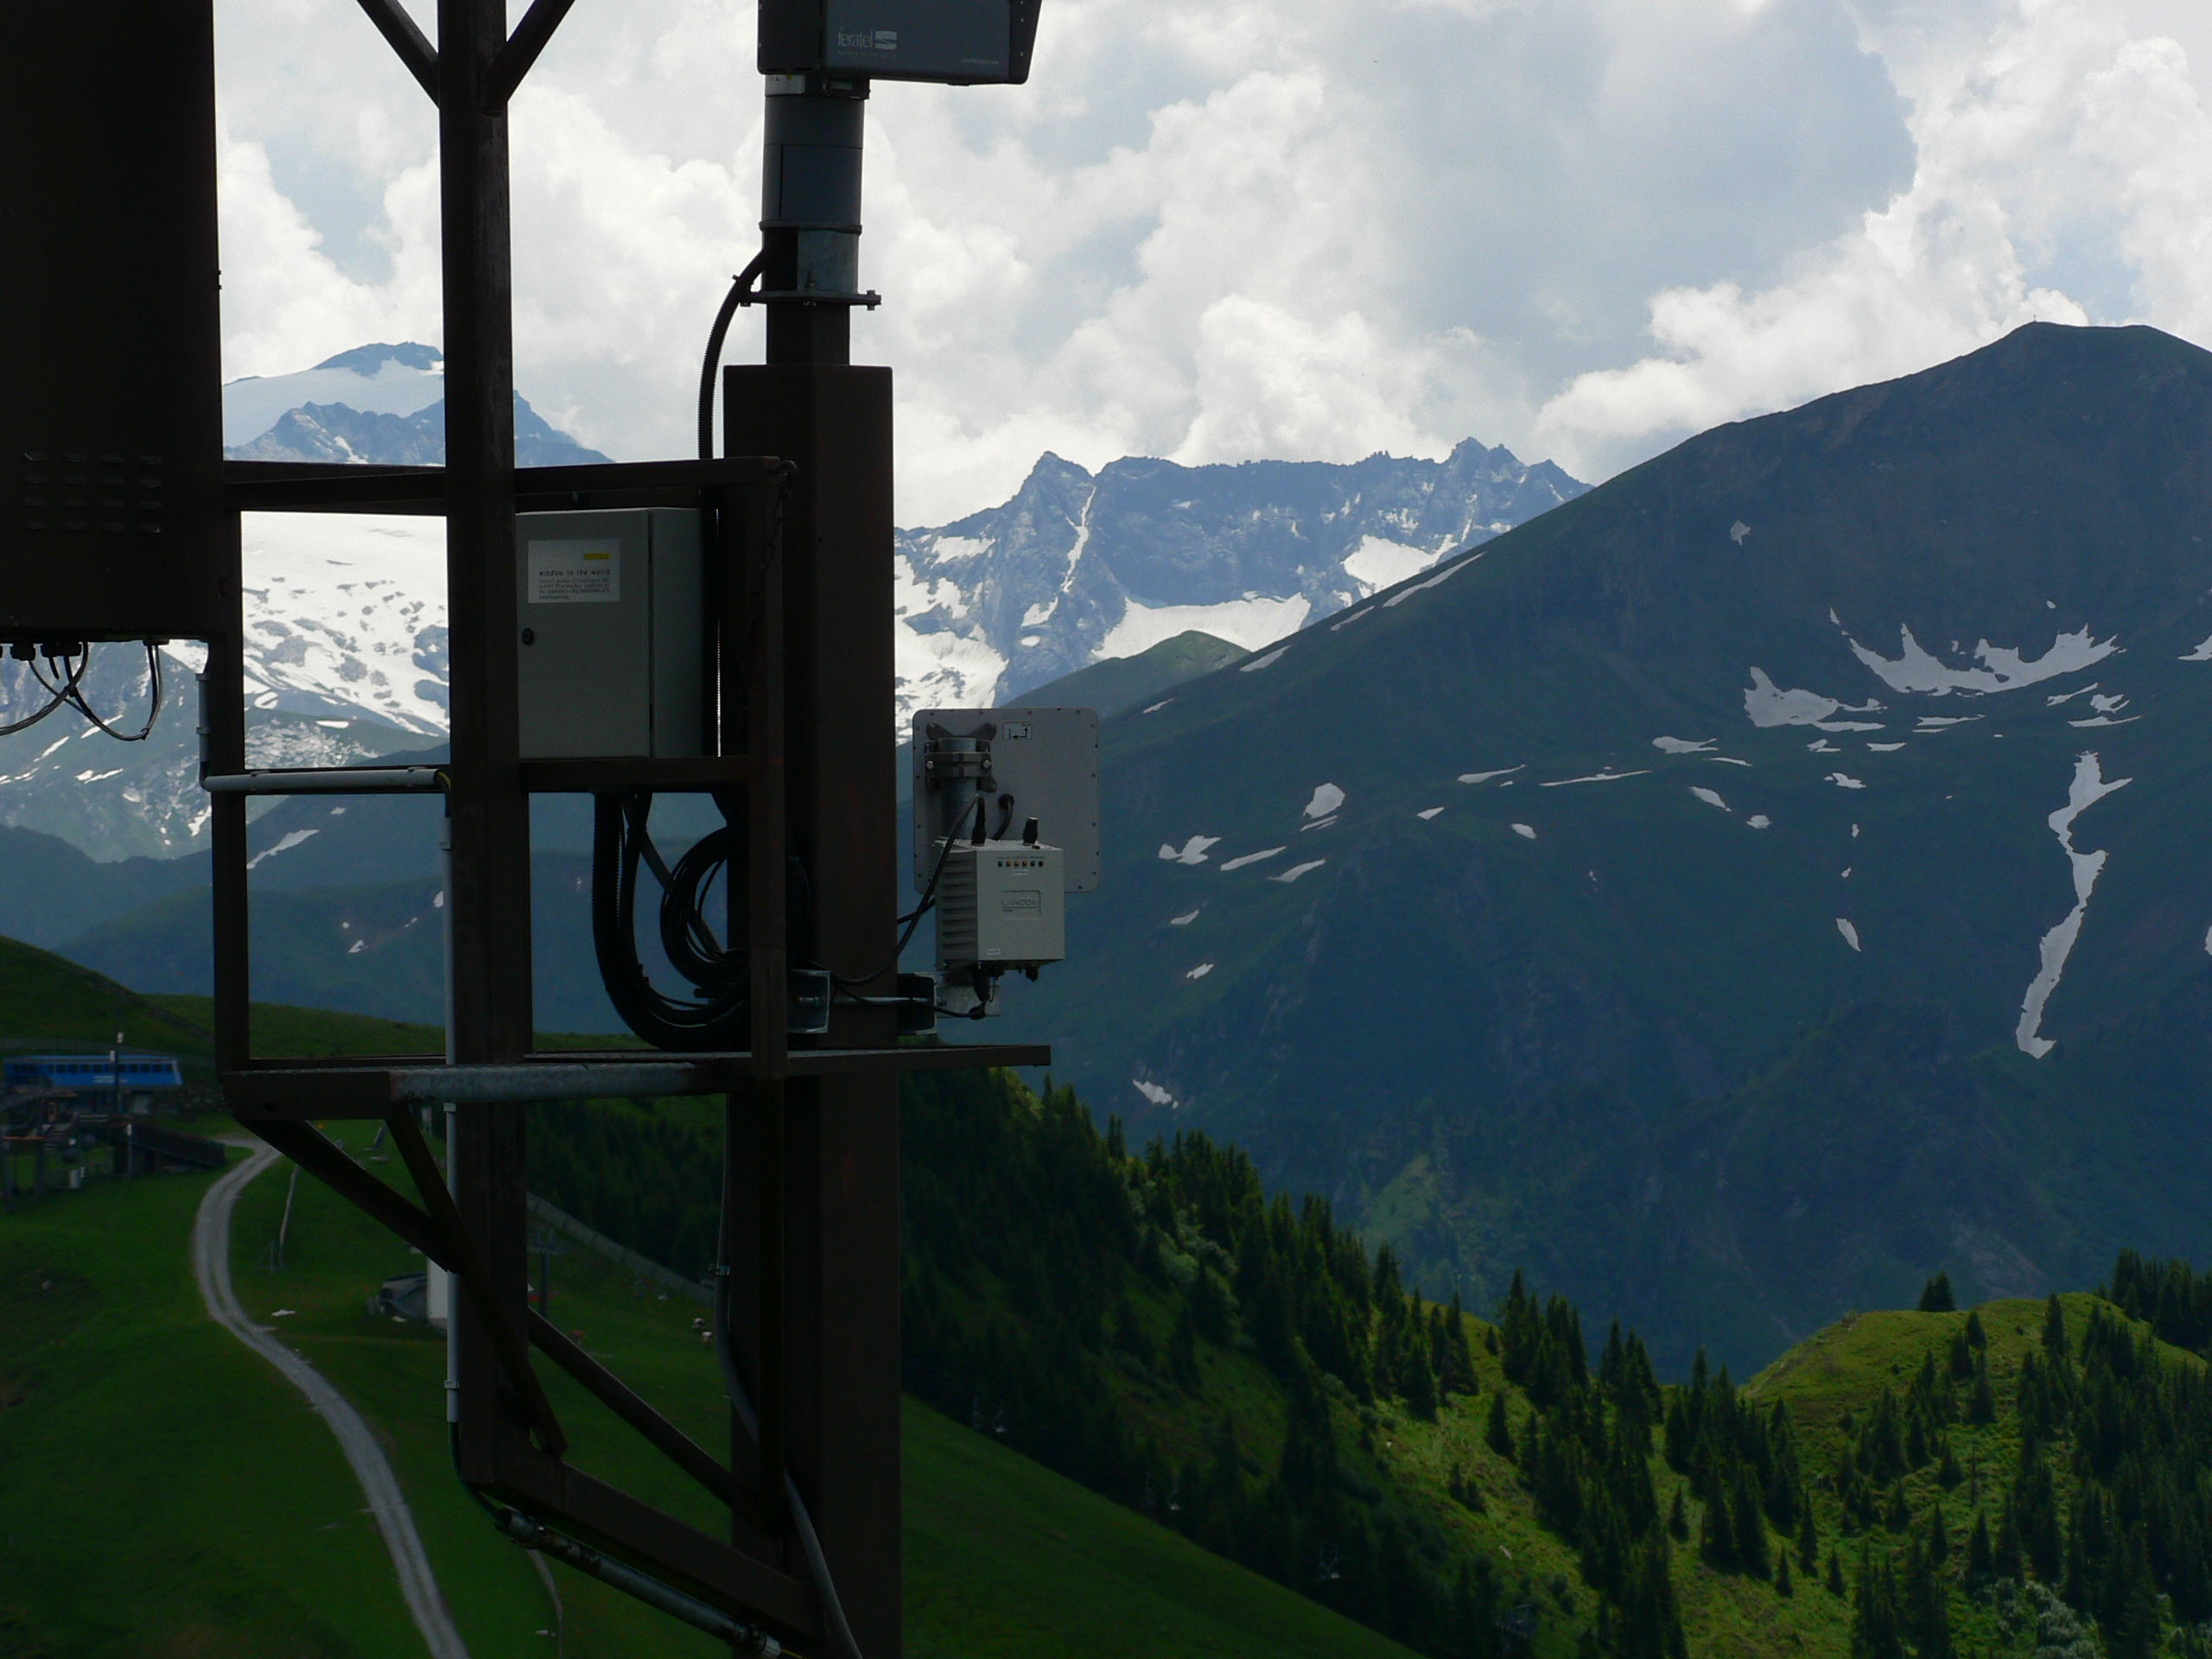
\includegraphics[width=0.5\textwidth]{figures/outdoor_berge.JPG}
      }
      \caption{Indoor accesspoint (left) and an outdoor accesspoint deployed (right) \cite{lancom}}
      \label{fig:L-322agn}
    \end{figure}
     
  \subsection{\ac{WLAN} Channel}
    A \ac{WLAN} Channel as specified by IEEE 802.11 family uses a specific frequency-range in the \ac{UHF} or \ac{SHF} radio-scope in order 
    to digitally modulate data on carrier waves.
    This is done to transmit data from a Sender station to a receiver station and creates a link between them.
    \ac{WLAN} uses the two license-free frequency bands at 2.4Ghz and additionally certain bands at 5Ghz.
    As we can see in \ref{fig:wlan_channels}, certain channels have overlapping regions. 
    Two independent pairs of radios in the same area can communicate almost completely free of interference, if they use different, non-overlapping channels.
    Some accesspoints use channels with 40 Mhz bandwidth in order to further increase throughput with the drawback of creating more overlapping frequencies regions
    and therefore possibly creating sources of interference with for other channels.
    The overlapping regions are a problem especially in the 2.4Ghz band but with widened channels the 5Ghz band is also affected, although not as bad since per default
    channels do not overlap.
    
    \begin{figure}[h!]
      \centering
      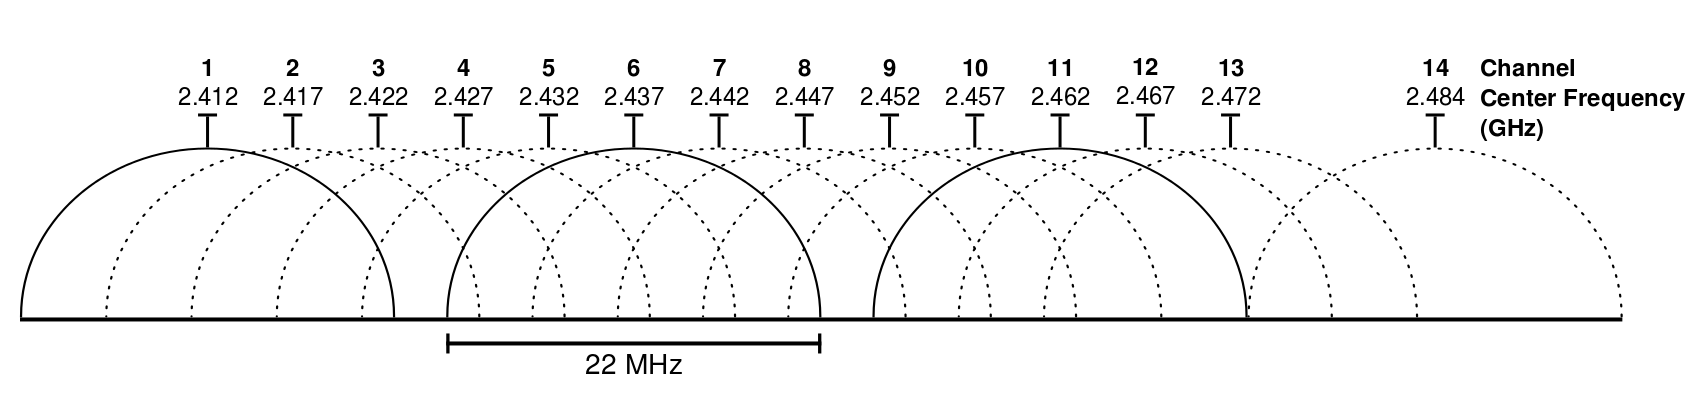
\includegraphics[width=0.8\columnwidth]{figures/wlan_channels.png}
      \caption{Mapping of channels to frequencies for the 2.4 Ghz band. \cite{wlan_channels}}
      \label{fig:wlan_channels}
    \end{figure}
    
      \subsubsection{\ac{CSMA/CA}}
	\ac{CSMA/CA} is a network protocol that describes how to access a shared medium, like a shared WLAN channel.
	It behaves as described by \cite{csma_techo}:
	\begin{quotation}
	  CSMA works on the principle that only one device can transmit signals on the network, 
	  otherwise a collision will occur resulting in the loss of data packets or frames. 
	  CSMA works when a device needs to initiate or transfer data over the network. 
	  Before transferring, each CSMA must check or listen to the network for any other transmissions that may be in progress. 
	  If it senses a transmission, the device will wait for it to end. Once the transmission is completed, 
	  the waiting device can transmit its data/signals. However, if multiple devices access it simultaneously and a collision occurs, 
	  they both have to wait for a specific time before reinitiating the transmission process. 
	\end{quotation}
	
	For a sizeable accesspoint-deployment the accumulated backoff-waiting times increase as more data is trasmitted and this backoff-timer is triggered more often.
	This effect also quickly degrades network performance in a mono-channel setup.
	
	Another interesting, but undesired problem in accessing the medium despite following the CSMA algorithm is the hidden-station-problem.
	It describes a scenario where an \ac{AP} B is in range of A and C but A and C do not see each other, see \ref{fig:csmaca}.
	If then the situation occurs that the two outer accesspoints simultaneously want to send data to the \ac{AP} in the middle, as they can not notice the 
	other accesspoint sending data, their packets collide at B and therefore effectively transmit less or nothing at all.
	The effect is the same like two people talking to one at the same time.
	To alleviate the problem the RTS/CTS extension was introduced, which introduces small \ac{RTS}-requests and \ac{CTS}-announcements. 
	This is basically the station/person that is talked to announcing to whom it is going to listen for the
	next period of time.
	
	\begin{figure}[th!]
	  \centering
	  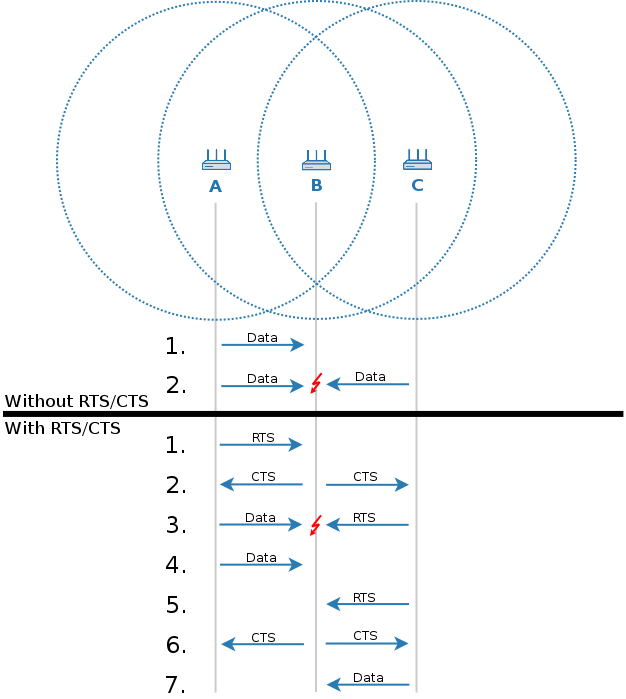
\includegraphics[width=1\columnwidth]{figures/csmaca.png}
	  \caption{Hidden-Station Problem and the RTS/CTS solution. A sends data to B in Step 1.
	    Because of the range-limitation, C does not recognize the transmission of A to B. 
	    If B then wants to also transmit data to B, it checks if the medium is free, which it falsely assumes
	    and then starts to transmit its data. This leads to collisions at B in step 2 and the data received will be corrupt.
	    First A asks B to send data to it, which B agrees on and sends the OK to everyone listening (A and C). 
	    Then A sends its data to B while C tries to get B\'s attention by requesting a CTS from it, which collidies with A's data and is ignored there.
	    Eventually C succeedes in getting its CTS and is able to also transmit its data to B without collisions.}
	  \label{fig:csmaca}
	\end{figure}

      \subsubsection{Interference}
	Wireless interference occurs if two sender at the same time transmit data on the same carrier frequency. If so the waves may interfere and be wrongly detected
	by the receiving stations. This leads to changed bits in the derived data and in turn to corrupt messages. Calculating the checksum on those packets will then 
	show that there have been errors while transmitting the data which will make the receiving station throw away this packet.
	As the receiving station will not acknowledge the receipt of the packet, the sender will assume the packet was not transmitted correctly and therefore try 
	to send the same packet again. If this process happens more often, throughput performance will suffer as it takes more time to send the same amount of data.
	This kind of interference is called of cooperative nature and occurs if two radios claim the same channel/medium (co-channel/adjacent-channel interference).
	Whereas there is also uncooperative interference from devices like microwaves or cordless phones which do not access the medium purposefully but rather
	emit noise by accident, nevertheless the effect is the same.
	
	For our purposes we define interference in wireless connections as any kind of disruption in communication, that includes both cooperative and non-coopertive interference.
	
	Despite solutions like RTS/CTS and others that mitigate the hidden station problem (and alleviate the cooperative interference),
	there are still some situations where collisions and therefore interference occurs.
	Additionally at a certain signal-strength level a station, while doing its carrier sensing, may not be able to differentiate noise from another stations transmission.
	As \cite{padhye2005estimation} mentions that interference is the key cause of performance degradiation in wireless networks, our goal is to increase throughput 
	performance by reducing interference as much as possible.
	
	\begin{figure}[h!]
	  \centering
	  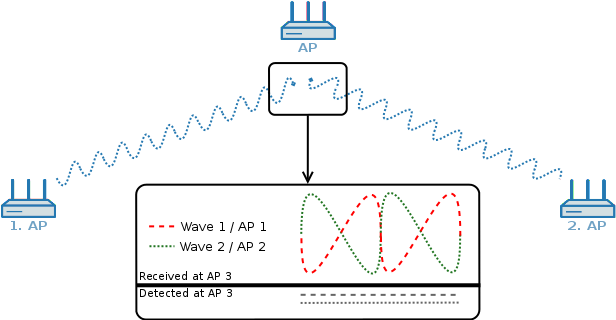
\includegraphics[width=0.8\columnwidth]{figures/interferenz}
	  \caption{When using the same carrier frequencies, waves may interfere and result in falsely detected bits and render the data corrupt.}
	  \label{fig:interferenz}
	\end{figure}
	      
    \subsection{Wireless Distribution System}
      \subsubsection{\ac{WLC}}
	The purpose of a \ac{WLC} is to manage and configure many accesspoints centrally and automatically - effectively ease the job of the administrator responsible for a 
	wireless infrastructure. They are usually located in central networking-cabinets next to other network core components like switches and servers.
	\begin{figure}[h!]
	  \centering
	  
\includegraphics[width=0.8\columnwidth]{figures/wlc}
	  \caption{A Lancom \ac{WLC}}
	  \label{fig:wlc}
	\end{figure}
      
      \subsubsection{WLC Aided Configuration}
	For a common WLAN infrastructe deployment all accesspoints are connected to the wired backbone and use their radios in infrastructe mode to 
	offer clients an entry point into the network.
	\begin{figure}[h!]
	  \centering
	  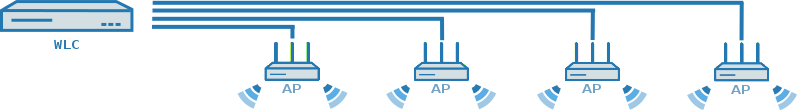
\includegraphics[width=0.8\columnwidth]{figures/wlc_aps}
	  \caption{Common accesspoint deployment. Accesspoints connected to backbone via wire.}
	  \label{fig:wlc_aps}
	\end{figure}
	The procedure of establishing such a network are as follows:
	\begin{enumerate}
	 \item Accesspoints search for a \ac{WLC} on the wired network by IP broadcast.
	 \item After authentication of the \ac{AP}, the \ac{WLC} responds and establishes a secure channel to the \ac{AP} through a \ac{CAPWAP}-Layer.
	 \item \ac{AP} receives a configuration from the \ac{WLC} through the secure channel and reconfigures itself accordingly.
	\end{enumerate}
	
      \subsubsection{Automatic \ac{WDS}}
      AutoWDS is then an extension to the WLC aided configuration by also allowing such a configuration procedure over wireless links instead of solely wired connections.
            
      \begin{figure}[h!]
	  \centering
	  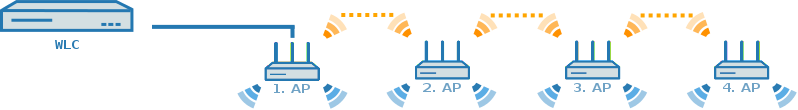
\includegraphics[width=0.8\columnwidth]{figures/autowds}
	  \caption{Autowds configuration setup. Only a few accesspoints are connected to the backbone via wire. 
	  Other accesspoints use their radios to connect to accesspoints that are connected to backbone via wire (first \ac{AP}) or relay accesspoints(second \ac{AP}).}
	  \label{fig:autowds}
      \end{figure}
      The procedure is enhanced accordingly:
      \begin{enumerate}
       \item The first \ac{AP} finds a WLC and proceeds as usual. Additionally it announces its connection to the WLC over its radios to other accesspoints.
       \item The second \ac{AP} does not find a \ac{WLC} on its LAN inferface and extends its search on the radios where it receives the announce of the first \ac{AP}.
	On its other radios it offers its services to clients.
       \item The second \ac{AP} establishes a secure connection (\ac{DTLS}) to the first \ac{AP} and continues its search for a \ac{WLC} over this link, 
	where it find the \ac{WLC} and also receives a configuration and proceeds as \ac{AP} one.
	\item Gradually all the accesspoints connect each other to the backbone and receive a configuration.
      \end{enumerate}

	
\section{Graph-theoretic Basics}
  A graph in graphtheory is a set of nodes and edges between those nodes. 
  
  A directed graph/digraph has directions on its edges defined.
  
  A weighted graph has weights attached to its edges.
  
  A graph is called connected if every pair of nodes is connected. 
  Two nodes a,b are connected if there exists a path from a to b.
  A path is a sequence of edges where each edge has to fit to the next, like in the game of domino.
  
  \begin{figure}[th!]
    \centering
    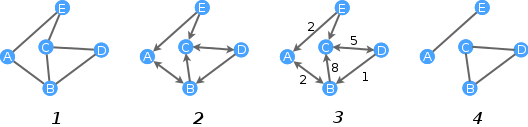
\includegraphics[width=0.8\columnwidth]{figures/graphen.png}
    \caption{Example graphs - 1: undirected 2: directed 3:weighted, directed 4: disconnected}
    \label{fig:graphen}
  \end{figure}

  We chose to use graphtheory to represent our networks as structures for two reasons:
  \begin{itemize}
   \item We are able to express all and only the necessary data with elements of a graph, like
    accesspoints and modules by nodes, links between accesspoints with edges and signal to noise ratio with weightedness. 
   \item Graph theory is a well reseached field and a lot of problems in graphtheory can be solved efficiently and intuitively 
    as we will show later with the \ac{DJP} algorithm in \ref{fig:djp}.
  \end{itemize}
    
  \subsection{Minimum Spanning Tree}
    A spanning tree is a subgraph for a given graph which contains all nodes of the original graph, but only the necessary subset of edges which are needed to connect each vertice
    to the component. In order to find a minimum spanning tree for a non-negative weighted graph we use the DJP algorithm \cite{prim}\cite{jarnik}.
    It works as described by the following:
    \begin{enumerate}
     \item Initialize the minimum tree with a single, randomly chosen vertex from the given graph.
     \item For all edges originating the set of nodes in the minimum tree to nodes which have not been visited yet, select the edge with the lowest score and add it and its nodes 
      to the minimum tree.
     \item Repeat step two as long as not all vertices of the given graph are visited.
    \end{enumerate}
    \begin{figure}[th!]
      \centering
      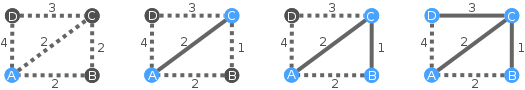
\includegraphics[width=0.8\columnwidth]{figures/djp.png}
      \caption{DJP algorithm calculating a minimal spanning tree.}
      \label{fig:djp}
    \end{figure}
    
  \subsection{k-vertex-connectivity, k-edge-connectivity}
    A graph is said to be \textit{k-vertex-connected} if there exists a set of \textit{k} vertices whose removal disconnects parts of the graph.\newline
    A graph is said to be \textit{k-edge-connected} if the graph is still connected after the removal of \textit{k} edges.
    \begin{figure}[th!]
      \centering
      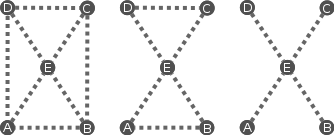
\includegraphics[width=0.5\columnwidth]{figures/connectivity.png}
      \caption{Graph-connectivity attributes from left to right: 1-vertex and 2-edge, 0-vertex and 1-edge, 0-vertex and 0-vertex}
      \label{fig:connectivity}
    \end{figure}
    
  \subsection{Mapping Data to Graph}
    For our purposes we will use the following mapping from devices and modules to a undirected, weighted graph.
    Each accesspoint and each module of our accesspoints is represented by a node.
    
    For each accesspoint we add edges with a special attribute "artificial" 
    to each module of its corresponding accesspoint and describe those edges as artificial or device-module-edges.
    Those edges also have their SNR value set to the maximum value possible. 
    
    If two modules are within receive range of each other, 
    we are adding an edge between the corresponding module nodes with the average signal-to-noise ratio as the edge-weight.
    We call those edges module-module connections or real connections.
    Since the average of the two SNR values might not describe all scenarios well enough (in a scenario where SNR values differ broadly),
    we easily can adjust the edge-weight to the minimum or maximum of those values.
    
    Furthermore we ignore onesided connections, i.e. one module receives one or a few beacons of the other module but not the other way round.
    Not only are the SNRs of those connections mostly very low/poor, but they are also very rare in our target scenarios with omnidirectional antennas.
    So mostly either the modules receive each others beacons, or both do not.
    \begin{figure}[th!]
      \centering
      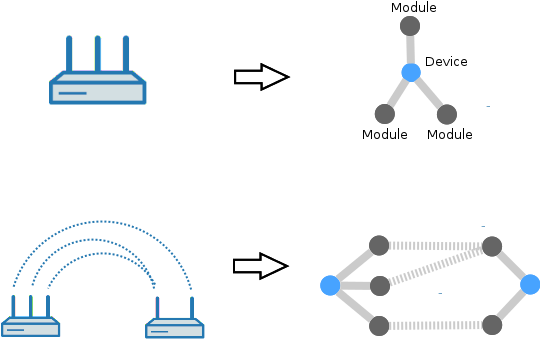
\includegraphics[width=0.5\columnwidth]{figures/apgraph.png}
      \caption{Graph representation of one (upper) and two connected accesspoints(lower)}
      \label{fig:apgraph}
    \end{figure}
    
  \subsection{Relevance of COLORING}
    Other pursuits on this problem including \cite{BFS-CA}, \cite{CTA}, \cite{caa_tricky} and \cite{katzela} mention a kinship to the problem COLORING on graphs.
    On the other hand \cite{caa_tricky} also mentions:
    \begin{quote}
     At first glance, this problem appears to be a graph-coloring problem. However, standard graph-coloring algorithms cannot really capute the specification and constraints 
     of the channel assignment problem. A node-multi-coloring formulation fails to capture [...] communicating nodes need[ing] a common color. On the other hand,
     an edge-coloring formulation fails to capture the [...] constraint where no more than \textit{q} (number of NICs per node) colors can be incident to a node.
     While a constraint edge-coloring might be able to roughly model the remaining constraints, it is incapable of satisfying the constraint of limited channel capacity.
    \end{quote}
    In addition to the modeling problems, a potential result of such a COLORING solution still would not make a point on the topology to use,
    as COLORING works on given network graphs and therefore topolgies, but we also have to decide how to create and select the network topology.
    As a consequence this formal problem considered in our work.
